\chapter{Competition}\label{ch:competition}

\section{How to read the table}\label{sec:comp-read}

Table~\ref{tab:vendors} lists what each vendor says about itself on its own public pages, which we read on 18 November 2026. Everything in it is a vendor claim, and none of it is independent evidence. A cell that reads ``not stated'' means that the page we could read does not say; it does not mean that the vendor lacks the feature. Prices are left out of the table because none of these vendors publishes one for its retail product; Chapter~\ref{ch:business} discusses the one public price list. Pages change, so the table is a snapshot.

\begin{table}
\caption{Vendor claims, as stated by the vendors (a snapshot)}\label{tab:vendors}
\begin{tabularx}{\textwidth}{lXX}
\toprule
\ctheaderrow\cthead{Vendor} & \cthead{What the vendor states} & \cthead{Shopper input}\\
\midrule
True Fit \cite{truefit_web} & fit and sizing intelligence, built on 20 years of purchase and return outcomes & purchase and return history; scanning not mentioned\\
Fit Analytics \cite{fitanalytics_web} & machine-learning size and fit recommendations & preferences, sales and returns records, a database of body scans\\
3DLOOK \cite{threedlook_web} & body scanning embedded by API or SDK; over 80 measurements in under 45 seconds & two guided smartphone photos \cite{threedlook_pricing}\\
Bold Metrics \cite{boldmetrics_web} & over 50 points of measure matched to the retailer's garment data & 4 to 6 simple inputs; no scanning, photos or tape\\
MySize \cite{mysize_web} & omnichannel platform with AI-driven apparel sizing & not stated\\
\midrule
Google \cite{google2023tryon} & generative-AI try-on on real models, sizes XXS to 4XL & a clothing image\\
Walmart and Zeekit \cite{walmart2021zeekit} & shoppers see themselves in a garment & uploaded photo or chosen model\\
\bottomrule
\end{tabularx}
\end{table}

\section{Direct vendors}\label{sec:comp-direct}

The direct field splits on one question: does the shopper scan, give a few inputs, or give nothing? True Fit sells to retailers and turns purchase-and-return outcomes into guidance, and its page does not mention body scanning \cite{truefit_web}. Fit Analytics states that it combines shopper preferences, sales and returns records with a database of body scans, so scans are reference data and not a shopper step \cite{fitanalytics_web}. 3DLOOK states that it embeds phone-based body scanning into a web page or app through an API, and its price list shows the cost of such scans \cite{threedlook_web,threedlook_pricing}. Bold Metrics takes the opposite position, stating that it needs no scanning, photos or measuring tape and works from four to six simple inputs \cite{boldmetrics_web}.

MySize is the one direct competitor at home. According to its annual report for 2022, the company is incorporated in Delaware, lists on the Nasdaq Capital Market and has its principal executive offices in Airport City, Israel \cite{mysize10k2022}. Its public page describes an omnichannel platform with AI-driven apparel sizing and says nothing we could check about scanning or price \cite{mysize_web}. We did not check whether the address has changed since 2022.

\section{Platform and in-house threats}\label{sec:comp-platform}

Large platforms are a different kind of threat. Google announced in 2023 a generative model that takes one clothing image and shows how it would drape on real models in sizes from XXS to 4XL \cite{google2023tryon}, and Walmart announced in 2021 a plan to acquire Zeekit, which lets customers see themselves in a garment from an uploaded picture or a chosen model \cite{walmart2021zeekit}. These tools visualize a garment, which is different from recommending a size, but a retailer that already has free visualization may feel that it does not need a vendor. We have not verified the later status of the Walmart plan.

\section{Positioning}\label{sec:comp-position}

Figure~\ref{fig:f2} places the vendors on two axes: whether the size comes from a questionnaire or size chart or from a body scan, and whether the product is a consumer app or a plug-in sold to retailers. ClosetTwin's chosen corner, a scan combined with garment specifications and fit preference, delivered as a plug-in to retailers, is not occupied by any vendor in the table. This proves only that the vendors do not say they occupy it; 3DLOOK, for one, could add the other inputs.

\begin{figure}
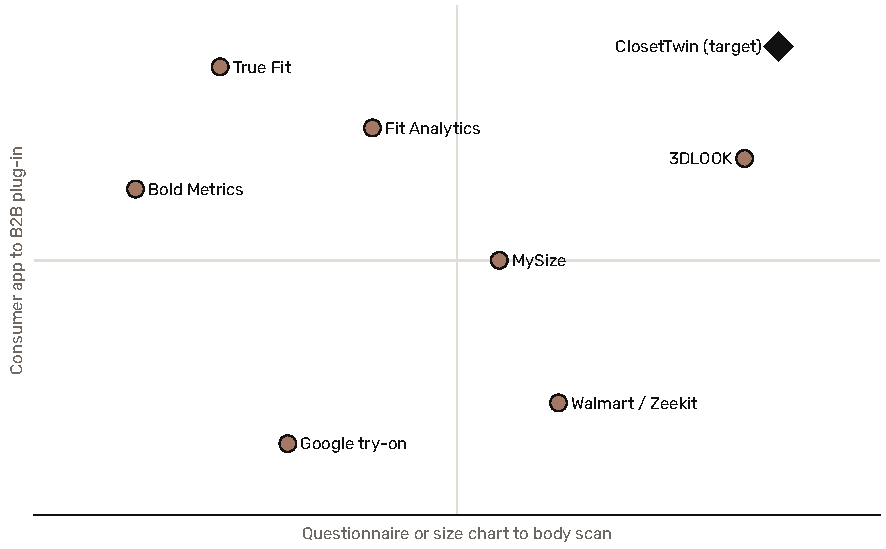
\includegraphics[width=\textwidth]{figures/f2-positioning.pdf}
\caption{Positioning of the vendors, our reading of vendor pages: source of the size input and type of product}\label{fig:f2}
\end{figure}

\section{The moat: proven, plausible or hypothesis}\label{sec:comp-moat}

We tag each claimed advantage honestly. That the combined input of scan, garment data and preference is better than any one of them is a \emph{hypothesis}: Peng and Duraffourg found that fit preference significantly affects the size people choose and that knowing the 3D shape alone is not enough for an efficient size recommendation \cite{peng2023}, which supports the combination but does not show that our implementation is better. That ClosetTwin lowers returns is a \emph{hypothesis until the pilot}. The counter-argument is real and we state it: Bold Metrics claims to match a shopper to garment data without a scan \cite{boldmetrics_web}, so a scan is an advantage only if it measurably improves the recommendation. Our edge in the early years is therefore a position and a test, not a moat.

\ctchapterend
